%
% kurven.tex -- Krümmung eines eindimensionalen Raumes, Einbettung
%
% (c) 2017 Prof Dr Andreas Müller, Hochschule Rapperswil
%
\chapter{Kurven%
\label{skript:kruemmung:section:kurve}}
\lhead{Kurven}
\rhead{}
Das Konzept der Krümmung einer Kurve wird bereits im ersten Semester
in der Analysis eingeführt,
die Formeln dafür sollen in diesem Kapitel kurz in Erinnerung gerufen werden.
Wichtiger aber ist die Erkenntnis, dass eine Kurve nur eine sehr simple
innere Geometrie hat.
Nach Wahl eines Anfangspunktes definiert die Bogenlänge entlang der Kurve 
ein Koordinatensystem für die Kurve vollständig.
Die Krümmung der Kurve ist also eine Eigenschaft der Einbettung einer Kurve.

Diese innere Einfachheit von Kurven macht sie zu einem Werkzeug, mit
dem wir später höherdimensionale Räume untersuchen können.
Wir können zum Beispiel Dreiecke in einer Fläche untersuchen,
und werden dabei erkennen, dass die Winkelsumme Auskunft geben kann
über die Krümmung der Fläche.
Die Krümmung einer Fläche ist also eine innere Eigenschaft, die mit
Hilfe von Experimenten mit Kurven erforscht werden kann.

\section{Länge einer Kurve}
\rhead{Definitionen}
Wir betrachten eine Kurve in der Ebene durch einen Parameterdarstellung
\[
c\colon [a,b] \to\mathbb R^2:t\mapsto c(t).
\]
Darin ist $c(t)$ als Vektor in der Ebene zu betrachten selbst wenn
wir dies nicht explizit durch Vektorpfeile anzeigen.
Man kann die Parametrisierung als die Wahl eines Koordinatensystems
für die Kurve interpretieren.
Es stellt sich daher die Frage, inwieweit Aussagen über die Kurve von
der Wahl dieses Koordinatensystems abhängig sind.

Alle unsere Untersuchungen werden die Analysis als Werkzeug verwenden,
wir wollen daher nur Kurven verwenden, für die eine ausreichend glatte
Parametrisierung vorliegt.
Wir verlangen daher, dass die Parameterisierung nach genügend oft nach
dem Parameter abgeleitet werden kann.
Die Ableitung 
\[
v(t)
=
\frac{dc(t)}{dt}
=
\dot c(t)
\]
ist ein Vektor, der im Punkt $c(t)$ tangential ist an die Kurve 
(Abbildung~\ref{skript:kurve:tangente}).
\begin{figure}
\centering
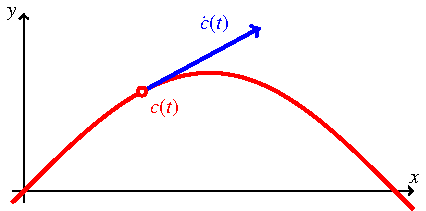
\includegraphics{chapters/tikz/tangente.pdf}
\caption{Kurve $c(t)$ parametrisiert mit dem Parameter $t$ und Tangentialvektor
$\dot c(t)$
\label{skript:kurve:tangente}}
\end{figure}

In $\mathbb R^2$ haben wir eine Längenmessung zur Verfügung, welche
wir dazu verwenden können, die Länge der Kurve zu berechnen.
Dazu betrachten wir zwei benachbarte Punkte $c(t)$ und $c(t+\Delta t)$
der Kurve.
Ihre Entfernung ist $|c(t+\Delta t) - c(t)|$.
Um daraus die Länge der Kurve zu berechnen, müssen wir die Kurve
an den Stellen $t_1,t_2,\dots,t_n$
beliebig fein in Teile aufteilen, und die Längen der Teilstrecken
auf addieren.
Die Summe
\[
l\simeq\sum_{k=1}^{n-1} |c(t_{i+1})-c(t_i)|
\]
ist daher eine Approximation für die Länge der Kurve.
Die Differenzen können wir mit Hilfe der Ableitung durch
\[
c(t_{i+1})-c(t_i) = \dot c(t_i)\cdot (t_{i+1}-t_i)
\]
approximieren.
Beim Grenzübergang zu einer beliebig feinen Unterteilung wird daraus
das Integral
\begin{equation}
l=\int_a^b |\dot c(t)|\,dt.
\end{equation}
Die Funktion
\begin{equation}
s(t)
=
\int_a^t |\dot c(\tau)|\,d\tau
\end{equation}
berechnet die Länge der Kurve zwischen den Parameterwerten
$a$ und $t$, wir wissen also insbesondere, dass $s(0)=0$.
$s(t)$ ist die {\em Bogenlänge} entlang der Kurve.
\index{Bogenlänge}

\section{Bogenlängenparameter}
\rhead{Bogenlängenparameter}
In diesem Abschnitt soll illustriert werden, dass wir bei der Wahl
einer Parametrisierung ein und derselben Kurve zwar viel Freiheit haben,
dass jedoch für geometrische Untersuchungen sich meistens gewisse
Parametrisierungen besonders eignen.
Sowohl hier als auch später beim Studium der Geodäten ist eine
Parametrisierung mit der Bogenlänge besonders nützlich.

\subsubsection{Ein Beispiel}
Wir betrachten die folgenden beiden Parametrisierungen einer ebenen Kurve:
\begin{equation}
\begin{aligned}
c_1\colon
[-1,1]\to\mathbb{R}^2
&\colon
t\mapsto\begin{pmatrix}x\\\sqrt{1-t^2}\end{pmatrix}
&&\text{und}&
c_2\colon
[0,\pi]\to\mathbb{R}^2
&
\colon
s\mapsto\begin{pmatrix}-\cos s\\\sin s\end{pmatrix}.
\end{aligned}
\end{equation}
Beide beschreiben den Einheitskreisbogen, der den Punkt $(-1,0)$ mit
dem Punkt $(1,0)$ verbindet (Abbildung \ref{skript:1dim:kreisbogen}).
Die Parametrisierungen unterscheiden sich aber in der Ableitung,
die Tangentialvektoren für die beiden Ableitungen sind
\begin{equation}
\begin{aligned}
\frac{dc_1}{dt}
&=
\begin{pmatrix}
1\\-\frac{1}{\sqrt{1-t^2}}
\end{pmatrix}
&&\text{und}&
\frac{dc_2}{ds}
&=
\begin{pmatrix}
\sin s\\\cos s
\end{pmatrix}.
\end{aligned}
\end{equation}
Der Tangentialvektor hat in der zweiten Parametrisierung konstant
die Länge $1$, während sie in der ersten Parametrisierung nahe bei
$t=\pm1$ über alle Grenzen wächst.
\begin{figure}
\centering
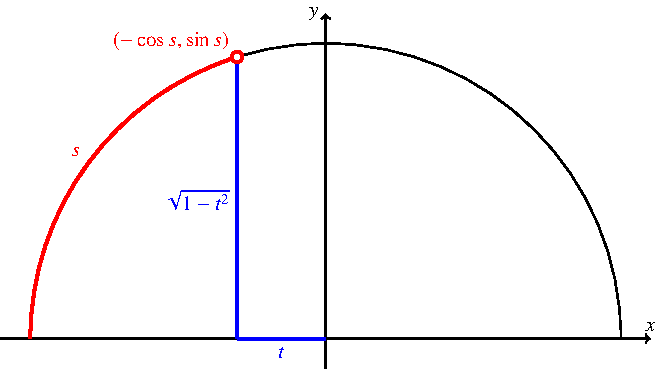
\includegraphics{chapters/tikz/kreisbogen.pdf}
\caption{Kreisbogen zwischen $(-1,0)$ und $(1,0)$. Im Text werden
zwei verschiedene Parametrisierungen dafür vorgestellt.
\label{skript:1dim:kreisbogen}}
\end{figure}

\subsubsection{Bestimmung der Bogenlänge}
Interpretieren wir den Parameter $t$ als die Zeit der Bewegung eines 
Teilchens entlang der Kurve, dann ist die zeitliche Änderung der Strecke,
die das Teilchen zurück gelegt hat, gerade die Länge des
Geschwindigkeitsvektors, also
\[
\frac{d}{dt} s(t) = \biggl|\frac{d}{dt}c(t)\biggr| = |\dot c(t)|.
\]
Die Funktion $s(t)$ ist also die Lösung der Differentialgleichung
\begin{equation}
\dot s(t)=|\dot c(t)|
\quad
\text{ mit der Anfangsbedingung }\quad s(a)=0.
\label{skript:kruemmung:laengedgl}
\end{equation}
Da $|\dot c(t)|$ eine stetige Funktion ist, können wir nach allgemeinen
Sätzen der Theorie der gewöhnlichen Differentialgleichungen davon ausgehen,
dass diese Differentialgleichung eine eindeutig bestimmte Lösung hat.

Die Differentialgleichung \eqref{skript:kruemmung:laengedgl} kann 
durch Integrieren sofort gefunden werden, sie ist
\begin{equation}
s(t)
=
\int_a^t \dot s(\tau)\,d\tau
=
\int_a^t |\dot c(\tau)| \,d\tau
=
\int_a^t \sqrt{\dot x(\tau)^2 + \dot y(\tau)^2}\,d\tau,
\label{skript:kruemmung:laenge}
\end{equation}
wie man auch durch Ableiten nach $t$ sofort nachprüfen kann.

\subsubsection{Charakterisierung von Bogenlängenparametrisierung}
Verlangen wir von der Kurvenparametrisierung $c(t)$ zusätzlich,
dass $|\dot c(t)|\ne 0$ für alle Parameterwerte $t$, dann ist
$s(t)$ sogar eine streng monoton wachsende Funktion, insbesondere
kann sie invertiert werden.
Wir können daher zu jedem gegebenen Wert der Länge $s$ durch
Anwendung der inversen Funktion sofort einen Parameterwert $t$
finden, bei dem der Wert $s$ der Länge erreicht wird, also
$s(t)=s$.
Wir schreiben diesen Wert auch abkürzen als $t(s)$, dies ist eine
vereinfachte Notation für die inverse Funktion von $s(t)$.
Die Ableitung der Funktion $s(t)$ ist
\begin{equation}
\frac{d}{ds} t(s) = \frac{1}{\dot s(t(s))} = \frac1{|\dot c(t(s))|}
\label{skript:kruemmung:abllaengeinv}
\end{equation}
nach der Formel für die Ableitung der inversen Funktion.

Zu einer beliebigen differenzierbaren Kurve mit der Eigenschaft
$|\dot c(t)|\ne 0$ können wir also immer eine neue Parametrisierung
$c(s)=c(t(s))$ finden, welche die Eigenschaft hat, dass $s$ die
Länge entlang der Kurve gerade die Kurvenlänge ist, die durchlaufen
wird.
Wir nennen $s$ auch den {\em Kurvenlängenparameter} entlang der
Kurve.
\index{Kurvenlängenparameter}
Wir sagen auch, $c(s)$ ist durch Kurvenlänge parametrisiert.

Die neue Parametrisierung hat als ``Geschwindigkeitsvektor''
\[
\frac{d}{ds} c(s)
=
\frac{d}{ds} c(t(s))
=
\dot c(t(s)) \frac{d}{ds}t(s)
\]
seine Länge wird unter Verwendung von
\eqref{skript:kruemmung:abllaengeinv}
\[
\biggl|
\frac{d}{ds} c(s)
\biggr|
=
\biggl|\dot c(t(s))\frac1{|\dot c(t(s))|}\biggr|
=
1,
\]
bei Verwendung eines Kurvenlängenparameters wird der Tangentialvektor
immer ein Einheitsvektor sein.

Umgekehrt wird die Differentialgleichung \eqref{skript:kruemmung:laengedgl}
besonderes einfach, wenn $|\dot c(t)|=1$ ist, nämlich $\dot s(t)=1$ mit
der Lösung $s(t)=t$.
Die Bedingung $|\dot c(t)|=1$ charaktersiert also $t$ als einen
Kurvenlängenparameter.

\subsubsection{Beispiele}
\begin{beispiel}
Wir betrachten eine Gerade 
\[
c(t)=\vec p + t\vec v,\qquad \vec v\ne 0
\]
in der Ebene.
Wir legen $a=0$ willkürlich fest.
Die Differentialgleichung~\eqref{skript:kruemmung:laengedgl} für die
Kurven\-längen\-funktion $s(t)$ wird
\[
\dot s(t) = |\dot c(t)| = |v|
\]
mit der Lösung
\[
s(t)=|v|t.
\]
Da $v\ne 0$ ist $s(t)$ monoton wachsend, und wir können sofort nach
$t$ auflösen, es ist
\[
t(s)=\frac{s}{|\vec v|}.
\]
Setzen wir dies in die ursprüngliche Parametrisierung ein, erhalten
wir
\[
c(s)
=
c(s(t))
=
\vec p + t(s)\vec v
=
\vec p + \frac{s}{|\vec v|}\vec v
=
\vec p + s\frac{v}{|v|},
\]
Die Ableitung nach $s$ hiervon ist ein Einheitsvektor, wie zu erwarten
war.
\end{beispiel}

\begin{beispiel}
Wir parametrisieren den Einheitskreis mit Hilfe der $x$-Koordinate, also
durch
\[
c\colon
[-1,1]\to\mathbb R^2
\colon
t\mapsto (-t,\sqrt{1-t^2}).
\]
Ganz offensichtlich ist dies kein Kurvenlängenparameter.
Für die Kurvenlänge brauchen wir die Ableitung nach dem Parameter $t$,
sie ist
\[
\dot c(t)=\biggl(-1, -\frac{t}{\sqrt{1-t^2}}\biggr).
\]
Die Kurvenlänge ist das Integral der Länge der Ableitung:
\[
s(t)
=
\int_{-1}^t \sqrt{1 + \frac{\tau^2}{1-\tau^2}}\,d\tau
=
\int_{-1}^t \sqrt{\frac{1-\tau^2 +\tau^2}{1-\tau^2}}\,d\tau
=
\int_{-1}^t \frac{1}{\sqrt{1-\tau^2}}\,d\tau
\]
Das Integral auf der rechten Seite kann man aber in geschlossener
Form auswerten, es ist
\[
s(t)=\arcsin(t) + \frac{\pi}{2}
\]
mit der inversen Funktion
\[
t(s)
=
\sin\biggl(s-\frac{\pi}2\biggr)
=
-\cos(s)
\]
Setzen wir dies in die Parametrisierung ein, erhalten wir
\[
c(s)
=
\bigl(\cos(s), \sqrt{1-\cos^2(s)}\bigr)
=
(\cos(s), \sin(s)),
\]
also die übliche Parametrisierung des Einheitskreises mit Hilfe
des Winkels.
Der Winkel muss in Bogenmass gemessen werden, also der Länge entlang
des Kreises.
\end{beispiel}

Da sich jede beliebige Kurve mit einem Bogenlängenparameter versehen
lässt, können wir für je zwei beliebige Kurven immer eine Abbildung
zwischen den Kurven definieren, die Punkte mit gleichem Bogenlängenparameter
zur Deckung bringt.
Zwei Kurven sind also nicht mehr unterscheidbar, wenn sie mal mit
einem Bogenlängenparameter ausgestattet sind.
Verbleibende Unterschiede zwischen Kurven entstehen einzig durch die
Einbettung der Kurve im Raum.

Für eine Ameise, die ausschliesslich auf der Kurve lebt, ist die Länge,
die sie entlang der Kurve zurückgelegt hat, die einzige geometrische
Information, die ihr zugänglich ist.
Sie kann verschiedene Kurven im Raum nicht voneinander unterscheiden.

\section{Krümmung}
\rhead{Krümmung}
\begin{figure}
\centering
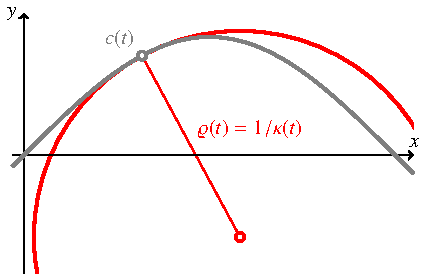
\includegraphics{chapters/tikz/kruemmung.pdf}
\caption{Krümmung $\kappa(t)$ und Krümmungsradius $\varrho(t)$
der Sinus-Kurve im Punkt $c(t)$
\label{skript:kurven:fig:kruemmung}}
\end{figure}
Wir möchten in diesem Abschnitt zeigen, dass die Krümmung einer Kurve
ausschliesslich eine Eigenschaft der Einbettung der Kurve in den
Raum ist.
Wir tun das, indem wir davon ausgehen, dass eine Kurve bereits mit
der Kurvenlänge parametrisiert ist, dass wir also die Standardparametrisierung
gewählt haben, in der über die innere Geometrie der Kurve verfügbare
Information bereits vollständig verwertet worden ist.

Eine Gerade zeichnet sich dadurch aus, dass der Tangentialvektor in
der Bo\-gen\-län\-gen\-pa\-ra\-me\-tri\-sie\-rung nicht ändert.
Eine Gerade ist nicht gekrümmt.
Krümmung ist also die Änderung des Tangentialvektors oder
\[
\kappa(s)=|\ddot c(s)|.
\]
\index{Krümmung einer Kurve}

\begin{beispiel}
Der Kreis mit Radius $r$ kann parametrisiert werden durch die Funktion
\[
s\mapsto c(s)=\biggl( r\cos\frac{s}{r}, r\sin\frac{s}{r}\biggr).
\]
Die Ableitung ist
\[
\dot c(s)=\biggl(-\sin\frac{s}{r},\cos\frac{s}{r}\biggr)
\qquad\Rightarrow\qquad
|\dot c(s)|
=
\sqrt{\cos^2\frac{s}{r}+\sin^2\frac{s}{r}}=1,
\]
dies ist also eine Parametrisierung mit Bogenlängenparameter.
Die Krümmung ist der Betrag der zweiten Ableitung, also
\[
\ddot c(s)=\biggl(-\frac1r\cos\frac{s}{r},-\frac1r\sin\frac{s}{r}\biggr)
\qquad\Rightarrow\qquad
\kappa(s)
=
|\ddot c(s)|
=
\frac1r.
\]
Der Kreis mit Radius $r$ ist also eine Kurve mit konstanter Krümmung
$\kappa(s)=\frac1r$.
\end{beispiel}

Ist die Kurve nicht durch die Bogenlänge parametrisiert, wird die
Berechnung der Krümmung etwas komplizierter.
Es muss aber immer noch gelten, dass $\kappa(t)$ die Änderung des
Einheitstagentialvektors pro Längeneinheit entlang der Kurve angibt.
Es ist also zu berechnen
\begin{equation}
\kappa(t)
=
\underbrace{\frac{1}{|\dot c(t)|}}_{\text{pro Längeneinheit}}
\cdot\;
\biggl|\frac{d}{dt}\underbrace{\frac{\dot c(t)}{|\dot c(t)|}}_{\text{Einheitstangentialvektor}}\biggr|.
\label{skript:kruemmung:krallg2}
\end{equation}
Die Berechnung ist etwas mühsam wegen des Vektorbetrages im Nenner.
Wir berechnen daher zuerst die Ableitung von $|\dot c(t)|$ mit
Hilfe der Kettenregel:
\begin{align*}
\frac{d}{dt}|\dot c(t)|
&=
\frac{d}{dt}\sqrt{\dot x(t)^2+\dot y(t)^2}
=
\frac1{2\sqrt{\dot x(t)^2 + \dot y(t)^2}}(2\dot x(t)\ddot x(t) + 2\dot y(t)\ddot y(t))
\\
&=
\frac{1}{|\dot c(t)|}
\begin{pmatrix}\dot x(t)\\\dot y(t)\end{pmatrix}
\cdot
\begin{pmatrix}\ddot x(t)\\\ddot y(t)\end{pmatrix}
=
\frac{1}{|\dot c(t)|}
\dot c(t)\cdot\ddot c(t)
=
\frac{\dot c(t)}{|\dot c(t)|} \cdot\ddot c(t).
\end{align*}
Damit können wir jetzt auch die Ableitung des Einheitstangentialvektors
berechnen:
\begin{align}
\frac{d}{dt} \frac{\dot c(t)}{|\dot c(t)|}
&=
\frac{\displaystyle\ddot c(t) |\dot c(t)| - \dot c(t) \frac{d}{dt}|\dot c(t)|}{|\dot c(t)|^2}
=
\frac{\displaystyle\ddot c(t) |\dot c(t)| - \dot c(t) \frac{\dot c(t)}{|\dot c(t)|}\cdot \ddot c(t)}{|\dot c(t)|^2}
=
\frac{\displaystyle\ddot c(t) - \frac{\dot c(t)}{|\dot c(t)|} \left( \frac{\dot c(t)}{|\dot c(t)|}\cdot \ddot c(t)\right)}{|\dot c(t)|}
\label{skript:kruemmung:krallg1}
\end{align}
Schreiben wir den Einheitstangentialvektor
\[
\vec e(t)= \frac{\dot c(t)}{|\dot c(t)|},
\]
wird der Zähler etwas übersichtlicher zu
\[
\ddot c(t) - \frac{\dot c(t)}{|\dot c(t)|} \biggl( \frac{\dot c(t)}{|\dot c(t)|}\cdot \ddot c(t)\biggr)
=
\ddot c(t) - \vec e(t)\; \bigl(\vec{e}(t)\cdot \ddot c(t)\bigr).
\]
Da $\vec e(t)$ ein Einheitsvektor ist, ist
$\vec e(t) \;(\vec e(t)\cdot\ddot c(t))$ die Projektion des Vektors
$\ddot c(t)$ auf den Vektor $\vec e(t)$.
Der Nenner ist also die Komponenten von $\ddot c(t)$ senkrecht auf dem
Tangentialvektor.
Wir brauchen davon aber nur den Betrag, also die Höhe des Parallelograms
mit den Seiten $\vec e(t)$ und $\ddot c(t)$.
Diese können wir aber auch dadurch erhalten, dass wir den orientierten
Parallelogramminhalt berechnen, und durch die Länge der Grundseite
$\vec e(t)$ teilen, die aber ein Einheitsvektor ist.
Den Parallelogramminhalt können wir mit der Determinante berechnen:
\[
\biggl|\ddot c(t) - \frac{\dot c(t)}{|\dot c(t)|}
\biggl(\frac{\dot c(t)}{|\dot c(t)|} \cdot \ddot c(t)\biggr)\biggr|
=
\det \biggl(\frac{\dot c(t)}{|\dot c(t)|}, \ddot c(t)\biggr)
=
\frac1{|\dot c(t)|}\det (\dot c(t),\ddot c(t)).
\]
Daraus können wir jetzt auch eine Formel für die Krümmung zusammensetzen.
Zunächst müssen wir den Faktor $|\dot c(t)|$ im Nenner wieder
hinzufügen, den wir in~\eqref{skript:kruemmung:krallg1} gefunden hatten.
Ausserdem brauchen wir einen weiteren Faktor $|\dot c(t)|$ im Nenner
aus der Definition~\eqref{skript:kruemmung:krallg2}.
Damit wird die allgemeine Formel
\begin{equation}
\kappa(t)
=
\frac{\det(\dot c(t),\ddot c(t))}{|\dot c(t)|^3}
\label{skript:kruemmung:krkurveallg}
\end{equation}
für die Krümmung einer ebenen Kurve.


\begin{beispiel}
Wir berechnen die Krümmung einer Ellipse mit den Halbachsen
$a$ und $b$, und verwenden dazu die Parametrisierung mit Hilfe des
Zentriwinkels, also
\[
c
\colon
[0,2\pi]\to\mathbb R^2
\colon
t\mapsto c(t) = (a\cos t, b \sin t).
\]
Nach der Formel~\eqref{skript:kruemmung:krkurveallg} brauchen wir zunächst
die ersten beiden Ableitungen, diese sind
\begin{align*}
\dot c(t)
&=
(-a\sin t, b\cos t)
\\
\ddot c(t)
&=
(-a\cos t, -b\sin t)
\end{align*}
Die Determinante von $\dot c(t)$ und $\ddot c(t)$ ist
\[
\det(\dot c(t), \ddot c(t))
=
\left|\begin{matrix}
-a\sin t & -a \cos t\\
 b\cos t & -b \sin t
\end{matrix}\right|
=
ab\sin^2t+ab\cos^2 t
=
ab.
\]
Die Krümmung ist daher
\[
\kappa(t)
=
\frac{ab}{(a^2\sin^2 t + b^2 \cos^2 t)^{\frac32}}
\]
Da die Faktoren $\sin^2t$ und $\cos^2t$ im Nenner sich zu $1$ summieren,
steht in der Klammer im Nenner ein gewichteter Mittelwert von $a^2$
und $b^2$.
Die Extremwerte des Nenners sind daher $a^3$ und $b^3$, sie werden bei
$t=\pm\frac{\pi}2$ bzw.~$t\in\{0,\pi\}$ angenommen.
Nimmt man an, dass $a>b$ ist, dann wird die maximale Krümmung $t=0$ und
und $t=\pi$ erreicht, sie ist $ab/b^3=a/b^2$.
Die minimale Krümmung wird dagegen bei $t=\pm\frac{\pi}2$ angenommen,
sie ist $ab/a^3=b/a^2$.

Ein Kreis ist eine Ellipse, bei der $a$ und $b$ übereinstimmen, dann sind
die beiden Extremwerte gleich gross, nämlich
\[
\frac{a}{b^2}=\frac{r}{r^2}=\frac1r
\qquad\text{und}\qquad
\frac{b}{a^2}=\frac{r}{r^2}=\frac1r,
\]
wie wir früher bereits gefunden haben.
\end{beispiel}

Für eine Kurve in drei Dimension lässt sich das bei der Herleitung
der Formel~\eqref{skript:kruemmung:krkurveallg} für $\kappa(t)$
verwendete Argument fast unverändert übertragen.
Die einzige Änderung ist an der Stelle erforderlich, wo wir die Determinante
zur Berechnung des orientierten Volumens des Parallelograms verwendet
haben.
In drei Dimensionen muss stattdessen der Betrag des Vektorproduktes 
verwendet werden.
Die Krümmung einer Raumkurve in einer beliebigen Parametrisierung ist
daher
\begin{equation}
\kappa(t)
=
\frac{|\dot c(t)\times \ddot c(t)|}{|\dot c(t)|^3}.
\label{skript:kruemmung:krkurveallg3d}
\end{equation}
Dies ist natürlich identisch mit \eqref{skript:kruemmung:krkurveallg},
wenn man sich die Ebene der Kurve in einen dreidimensionalen Raum
eingebettet vorstellt.

\begin{beispiel}
\begin{figure}
\centering
\includegraphics[width=\hsize]{chapters/3d/kurve.jpg}
\caption{Kurven $t\mapsto(t,t^2,0)$ (rot) und $t\mapsto(t,t^2,t^3)$ (gelb).
\label{skript:kruemmung:fig:kurvekr}}
\end{figure}
Wir betrachten die beiden Kurven
\begin{align*}
c_1(t)&=(t,t^2,0)
&
c_2(t)&=(t,t^2,t^3)
\end{align*}
(Abbildgung~\ref{skript:kruemmung:fig:kurvekr}).
$c_1(t)$ ist eine ebene Kurve, nämlich die Projektion der Raumkurve
$c_2(t)$ in die $x$-$y$-Ebene, sie ist in
Abbildung~\ref{skript:kruemmung:fig:kurvekr} rot dargestellt.
Die Kurve $c_2(t)$ ist in Abbildung~\ref{skript:kruemmung:fig:kurvekr} 
dagegen gelb dargestellt.
Wir wollen von beiden Kurven die Krümmung berechnen.
Dazu berechnen wir zunächst die Ableitungen und das Vektorprodukt
\begin{align*}
\dot c_1(t)
&=
(1,2t,0)
&
\dot c_2(t)
&=
(1,2t,3t^2)
\\
\ddot c_1(t)
&=
(0,2,0)
&
\ddot c_2(t)
&=
(0, 2, 6t)
\\
\dot c_1(t)\times \ddot c_1(t)
&=
(0,0,2)
&
\dot c_2(t)\times \ddot c_2(t)
&=
(6t^2,-6t,2)
\end{align*}
Daraus kann man jetzt die Krümmungen berechnen:
\begin{align*}
\kappa_1(t)
&=
\frac{2}{(1+4t^2)^{\frac32}}
\\
\kappa_2(t)
&=
\frac{2}{(1+4t^2 + 9t^4)^{\frac32}}
\sqrt{1+9t^2+9t^4}
\end{align*}
Für den Parameterwert $t=0$ stimmen die beiden Krümmungen überein.
\end{beispiel}

\section{Rekonstruktion einer ebenen Kurve aus der Krümmung}
\rhead{Rekonstruktion aus der Krümmung}
Die Krümmung bestimmt eine Kurve eindeutig.
Um dies einzusehen, parametrisieren wir eine ebene Kurve mit
$x$, schreiben also $c(x)=(x,y(x))$.
Wir müssen jetzt nachrechnen, dass die Vorgabe der Krümmung $\kappa(x)$
und der Steigung in einem Punkt die Kurve eindeutig festlegt.
Dazu stellen wir eine Differentialgleichung zweiter Ordnung auf,
allgemeine Sätze über Existenz und Eindeutigkeit der Lösung von
gewöhnlichen Differentialgleichungen werden unsere Aussage dann
als Konsequenz haben.

In dieser speziellen Wahl der Parametrisierung ist $\dot x = 1$ und
$\ddot x=0$.
Die Ableitung von $y$ nach dem Parameter ist dann $\dot y=y'(x)$.
Somit wird die Formel für die Krümmung
\[
\kappa(x)
=
\frac{\left|\begin{matrix}\dot x&\ddot x\\\dot y&\ddot y\end{matrix}\right|}{(\dot x^2+\dot y^2)^{\frac32}}
=
\frac{\left|\begin{matrix}1&0\\y'&y''\end{matrix}\right|}{(1+y'^2)^{\frac32}}
=
\frac{y''}{(1+y'(x))^{\frac32}}
\]
der in expliziter Form:
\[
y''(x)=\kappa(x) (1+y'(x)^2)^{\frac32}.
\]
Dies ist eine gewöhnliche Differentialgleichung zweiter Ordnung.
Da die rechte Seite erfüllt die Bedingungen, die in üblichen
Eindeutigkeitssätzen für gewöhnliche Differentialgleichungen
verlangt werden, daher gibt es genau eine Lösung dieser
Differentialgleichung zu vorgegebenem Anfangspunkt und Anfangsrichtung.
Damit ist gezeigt, dass in der Ebenen zwei Kurven mit der gleichen
Krümmung, gleichem Anfangspunkt und gleicher Anfangsrichtung übereinstimmen
müssen.
Anders formuliert: zwei ebene Kurven mit gleicher Krümmung in Abhängigkeit
von einem Bogenlängenparameter sind kongruent.

In drei Dimensionen kann die Krümmung allein eine Raumkurve nicht bestimmen.
Man kann dies zum Beispiel so einsehen.
Ist $c(t)$ eine gegeben Raumkurve, dann können wir deren Krümmung
$\kappa(t)$ berechnen.
In jeder Ebene durch den Punkt $c(0)$, die auch den Tangentenvektor
$\dot c(t)$ enthält, gibt es eine ebenen Kurve mit der gleichen
Krümmung $\kappa(t)$.
Da es unendlich viele solche Ebenen gibt, gibt es unendlich viele 
ebene Kurven, die die gleiche Krümmung haben wie die vorgegebene
Raumkurve.

Um eine Raumkurve eindeutig festzulegen braucht es daher ein weiteres
Datum, welches beschreibt, wie sich die aktuelle Tangentialebene
aufgespannt von $\dot c(t)$ und $\ddot c(t)$ dreht.
Diese {\em Torsion} genannt Grösse bestimmt dann die Kurve vollständig.
\index{Torsion}
Für eine ebene Kurve verschwindget die Torsion.

Die Kurventheorie lässt sich sogar auf eine beliebig grosse Zahl
von Dimensionen verallgemeinern.
Es stellt sich heraus, dass mit jeder zusätzlichen Dimension eine
zusätzliche Funktion notwendig wird.
Für eine Kurve in $n$ Dimensionen braucht es also $n-1$ Funktionen,
die beschreiben, wie sich ein entlang der Kurve mitbewegtes Koordinatensystem,
das sogenannte Frenet-$n$-Bein ändert.
\index{Frenet-$n$-Bein}
Diese Funktionen legen dann die Kurve bis auf die Wahl einer Anfangslage
des Koordinatensystem eindeutig fest.
Mit anderen Worten, wenn zwei Kurven in $n$ Dimensionen in den genannten
$n-1$ Funtionen übereinstimmen, dann sind sie kongruent.

\section*{Übungsaufgaben}
\rhead{Übungsaufgaben}
\uebungsaufgabe{0101}

